%!TEX root = Thesis_David_Burns.tex
\chapter{Introduction}
\label{ch:intro}

% make sure that every chapter that appears in here is given some love.
% you want to give the reader a foresight into what is to come.
% lay out the progression of ideas for them.
% your last paragraph here should be one line descriptions of each of the main sections to come

Climate change is a global issue effecting every country on Earth. The contributions to climate change are varied and complex requiring in depth study to provide as precise a picture as possible. Changes in the Earth's energy balance result from radiative forcing. Radiative forcing is changes in the amount of radiative energy absorbed or reflected by the ground and atmosphere. The radiative forcing component that currently has the largest uncertainty is aerosols (see \cref{fig:radforc}) \citep{intergovernmentalpanelonclimatechange:2015fa}. Aerosols are particles suspended in the air that can directly scatter or absorb radiation, or cause water vapour to condense onto them, acting as cloud condensation nuclei (\gls{ccn}). Clouds formed from \gls{ccn} reflect radiation back into space. As such the exploration of aerosols as a radiative forcing mechanism is a key area in understanding the larger issue of climate change.

\begin{figure}[!htb]
 	\centering
 	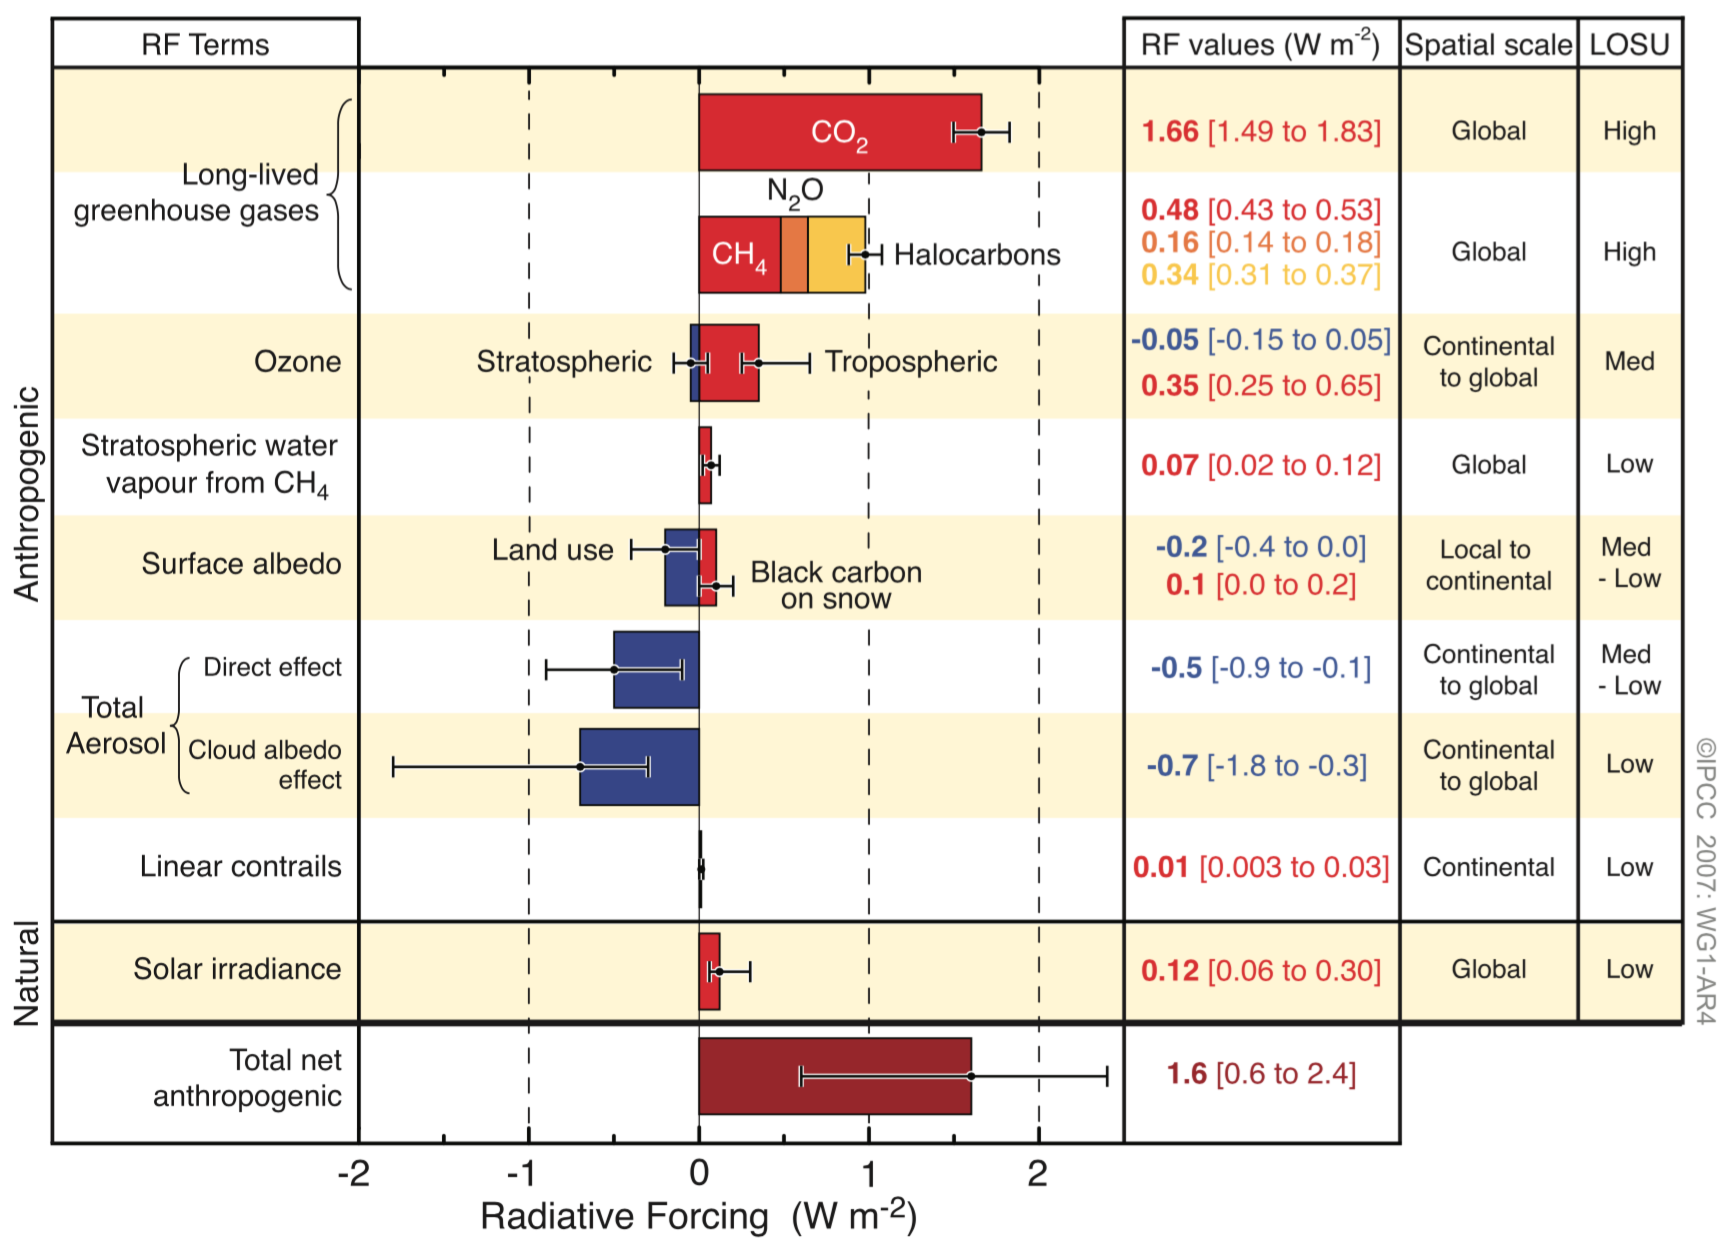
\includegraphics[width=0.8\textwidth,natwidth=1730,natheight=1248]{Fig/Radiative_Forcing.png}
 	\caption{A diagram illustrating the various influences on radiative forcing along with their associated uncertainties. From the 2015 Intergovernmental Panel on Climate Change. The largest contributor to uncertainty is currently aerosols \citep{intergovernmentalpanelonclimatechange:2015fa}.}
 	\label{fig:radforc}
\end{figure}

A major cause of these uncertainties is the necessity for regionally specific aerosol knowledge \citep{intergovernmentalpanelonclimatechange:2015fa}. Aerosol composition and concentration differs greatly with changes in sources and atmospheric conditions. This regional variation translates to variation in direct scattering/absorption and cloud producing potential, leading to both local and global effects on climate. Thus it is important to develop tested, regionally specific models that take into account these variations \citep{cainey:2007jj, simpson:2014}. 

In 1987 the \gls{claw} hypothesis was defined in the seminal paper `Oceanic phytoplankton, atmospheric sulphur, cloud Albedo and climate'. The abbreviation \gls{claw} was taken from the initials of that paper's authors, Robert Charlson, James Lovelock, Meinrat Andreae and Stephen Warren. They proposed a feedback mechanism where stress driven marine biota produced chemicals that influenced cloud cover \citep{charlson:1987fw}. This paper generated a vast body of research involving many disciplines. Dimethyl sulphide (\gls{dms}) is the core chemical responsible for the mechanism and is produced by phytoplankton, and as discovered more recently, coral \citep{raina:2013fj}. As the climate shifts towards increased temperature, regions like the Great Barrier Reef (\gls{gbr}) are increasingly losing coral coverage \citep{hoeghguldberg:1999bi}. It is therefore important to examine the potential effects on climate caused by \gls{dms} producing biota undergoing climate related reduction.

%maybe this needs to be moved to the conclusion?
Modelling \gls{dms} as it is produced, transformed and transported through the atmosphere, in the \gls{gbr} region, will provide needed insight into the mechanisms surrounding \gls{dms}. To do so requires a group of models simulating the different layers of the problem. The bottom most layer is \gls{csiro}'s Conformal-Cubic Atmospheric Model (\gls{ccam}) which provides information such as wind speed and temperature \citep{mcgregor:2005wz}. The middle layer is CSIRO's Chemical Transport Model (\gls{ctm}) which tracks chemical concentrations \citep{cope:2009tz}. The final layer is the Global Model of Aerosol Processes (\gls{glomap}) which simulates aerosol interactions and produces aerosol concentrations. This project will attempt to apply this trio of models, specifically targeting \gls{dms} in the \gls{gbr} region, and to analyse the results with potential for modelling future climate scenarios.

%Understanding the role of the CLAW hypothesis and its current position will provide the necessary foundational knowledge. Looking at the modelling system itself and other modelling studies will give greater clarity in our approach. The pathways \gls{dms} proceeds down to form cloud condensation nuclei (\gls{ccn}) involve complicated chemistry \citep{Barnes:2006ug} and must be examined to ensure we have the best knowledge of current theory to match with the model. Finally, a look at other regionally specific and global large scale studies is needed to form an overview of the problem.

Primarily, it is necessary to understand the role of the atmosphere and its constituents, and where aerosols and \gls{dms} are positioned within it. The pathways \gls{dms} proceeds down to form \gls{ccn} involve complicated chemistry \citep{barnes:2006ug} and must be explored to ensure the modelling mirrors current theory. The unique climatology of the \gls{gbr}, including the mechanism and scale with which coral contributes to \gls{dms}, needs to be established to provide localised inputs for the group of models. Modelling and the models themselves must be understood to ensure they are being applied correctly and to determine if they are sufficient for simulating the \gls{dms} to \gls{ccn} pathway. Finally, researching the method through which \gls{dms} enters the atmosphere, along with previous \gls{dms} to \gls{ccn} modelling attempts, provides insight into the modelling process and what areas of this research area remain unexplored.

%\section{Research Topic}


